% =====================================================================
%  MFE 230GA Final Project: "Follow the Workers". Report v1 (overnight build, 3-4 Oct 2026).
%  House template: preamble.tex. Conventions:
%    \tagc \tagp \tagf   label pill in every table and figure caption
%    % src: <file>      after every number (claim IDs refer to results/claims.csv)
%    \prov{...}         number not yet verified against a file
%    \todo{...}         content a human must write
%  Build: latexmk -pdf main.tex   (\draftfalse for the submission build)
% =====================================================================
% =====================================================================
%  House LaTeX template: minimal, light (Piero). Shared by report/ and results/.
% =====================================================================
\documentclass[11pt]{article}

% ---------- PAGE ----------
\usepackage[a4paper,margin=2.1cm,headheight=14pt,footskip=26pt]{geometry}
\setlength{\parindent}{0pt}
\setlength{\parskip}{0.55em}
\IfFileExists{lmodern.sty}{\usepackage[T1]{fontenc}\usepackage{lmodern}}{}
\usepackage{microtype}
\usepackage{amsmath,amssymb}
\linespread{1.04}

% ---------- COLOURS (Berkeley) ----------
\usepackage[dvipsnames]{xcolor}
\definecolor{bblue}{HTML}{003262}   % Berkeley Blue
\definecolor{bgold}{HTML}{FDB515}   % California Gold
\definecolor{ink}{HTML}{16181D}
\definecolor{mute}{HTML}{6B7280}
\definecolor{hair}{HTML}{D4D8DE}
\definecolor{paper}{HTML}{F5F6F8}
\definecolor{confc}{HTML}{003262}   % confirmatory
\definecolor{posthc}{HTML}{B35C00}  % post-hoc
\definecolor{fwdc}{HTML}{2E7D32}    % forward test
\color{ink}

% ---------- PACKAGES ----------
\usepackage{graphicx}
\usepackage{booktabs,tabularx,array,threeparttable,multirow}
\newcolumntype{Y}{>{\raggedright\arraybackslash}X}
\setlength{\aboverulesep}{0.3ex}\setlength{\belowrulesep}{0.5ex}
\usepackage{float}
\usepackage[font=small,labelfont={color=bblue,sc},labelsep=period,skip=5pt,justification=raggedright,singlelinecheck=false]{caption}
\usepackage{subcaption}
\usepackage[shortlabels]{enumitem}
\setlist{itemsep=1pt,topsep=2pt,parsep=0pt}
\usepackage{titlesec}
\usepackage{fancyhdr}
\usepackage[most]{tcolorbox}
\usepackage{listings}
\usepackage{tikz}
\usetikzlibrary{arrows.meta,positioning,calc}
\usepackage[round,authoryear]{natbib}
\usepackage[colorlinks=true,linkcolor=bblue,citecolor=bblue,urlcolor=bblue]{hyperref}
\usepackage[capitalise,noabbrev]{cleveref}

% ---------- REPORT INFO ----------
\newcommand{\ReportTitle}{Follow the Workers}
\newcommand{\ReportSubtitle}{Do labor-market flows predict which U.S.\ industries outperform?}
\newcommand{\CourseName}{MFE 230GA \textendash{} Equity Markets}
\newcommand{\CourseShort}{MFE 230GA}
\newcommand{\Term}{Fall 2026}
\newcommand{\SubmitDate}{October 4, 2026}

% ---------- SECTIONS (bold only in titles) ----------
\titleformat{\section}{\large\bfseries\color{bblue}}{\thesection}{0.7em}{}[{\color{hair}\titlerule[0.5pt]}]
\titlespacing*{\section}{0pt}{16pt}{8pt}
\titleformat{\subsection}{\normalsize\bfseries}{\textcolor{bblue}{\thesubsection}}{0.7em}{}
\titlespacing*{\subsection}{0pt}{11pt}{3pt}
\titleformat{\paragraph}[runin]{\normalsize\itshape}{}{}{}[.]
\titlespacing*{\paragraph}{0pt}{6pt}{0.6em}

% ---------- HEADER / FOOTER ----------
\pagestyle{fancy}\fancyhf{}
\renewcommand{\headrulewidth}{0pt}
\renewcommand{\footrulewidth}{0.4pt}
\renewcommand{\footrule}{{\color{hair}\hrule width\headwidth height\footrulewidth\vskip\footruleskip}}
\fancyhead[R]{\footnotesize\color{mute}Page \thepage}
\fancyfoot[L]{\footnotesize\color{mute}\CourseShort{} \textperiodcentered{} Final Project}
\fancyfoot[R]{\footnotesize\color{mute}\ReportTitle}

% ---------- LABELS, DRAFT MARKS ----------
\newif\ifdraft \drafttrue   % \draftfalse for the submission build
\DeclareRobustCommand{\pill}[2]{\tcbox[on line,colback=#1!9,colframe=#1!9,boxrule=0pt,arc=1.6pt,
  left=2.5pt,right=2.5pt,top=0.5pt,bottom=0.5pt,boxsep=0pt]{\textcolor{#1}{\scriptsize\textsc{#2}}}}
\DeclareRobustCommand{\tagc}{\pill{confc}{confirmatory}}
\DeclareRobustCommand{\tagp}{\pill{posthc}{post-hoc}}
\DeclareRobustCommand{\tagf}{\pill{fwdc}{forward test}}
\newcommand{\prov}[1]{\ifdraft{\setlength{\fboxsep}{1pt}\colorbox{bgold!30}{#1}}\else #1\fi}
\newcommand{\todo}[1]{\ifdraft{\color{red!70!black}\footnotesize[TODO: #1]}\fi}

% ---------- BOXES ----------
\newtcolorbox{keybox}[1][]{enhanced,breakable,sharp corners,frame hidden,boxrule=0pt,
  colback=paper,borderline west={2pt}{0pt}{bgold},left=9pt,right=9pt,top=5pt,bottom=6pt,
  fontupper=\small,before upper={\ifx\relax#1\relax\else{\textcolor{bblue}{\textsc{#1}}\par\smallskip}\fi}}
\newtcolorbox{promptbox}[1]{enhanced,breakable,sharp corners,frame hidden,boxrule=0pt,
  colback=paper,borderline west={2pt}{0pt}{bblue},left=9pt,right=9pt,top=5pt,bottom=6pt,
  before upper={{\small\textcolor{bblue}{\textsc{#1}}}\par\smallskip\raggedright\footnotesize\ttfamily}}

% ---------- CODE ----------
\lstset{language=Python,basicstyle=\ttfamily\footnotesize,columns=fullflexible,keepspaces,
  breaklines,showstringspaces=false,frame=leftline,framerule=2pt,rulecolor=\color{bblue},
  backgroundcolor=\color{paper},xleftmargin=8pt,framexleftmargin=8pt,aboveskip=6pt,belowskip=6pt,
  keywordstyle=\color{bblue},commentstyle=\color{mute}\itshape,stringstyle=\color{posthc}}

% ---------- COVER ----------
\newcommand{\BerkeleyMark}{%
  \IfFileExists{figures/berkeley_mfe_logo.pdf}{\includegraphics[height=1.4cm]{figures/berkeley_mfe_logo.pdf}}{%
  \IfFileExists{figures/berkeley_mfe_logo.png}{\includegraphics[height=1.4cm]{figures/berkeley_mfe_logo.png}}{%
  {\color{bblue}\fontsize{24}{26}\selectfont\bfseries Berkeley}\hspace{0.7em}%
  {\color{bgold}\rule[-3pt]{1.4pt}{22pt}}\hspace{0.7em}%
  \parbox[b]{7cm}{\color{bblue}\footnotesize\textsc{Haas School of Business}\\[-1pt]\textsc{Master of Financial Engineering}}}}}

\newcommand{\MakeCover}{%
\begin{titlepage}
\newgeometry{margin=2.5cm}
\BerkeleyMark
\vspace*{0.26\textheight}

{\raggedright
{\color{mute}\small\textsc{\CourseShort{} \textperiodcentered{} Final Project \textperiodcentered{} \Term}}\par\vspace{10pt}
{\fontsize{34}{38}\selectfont\bfseries\color{bblue}\ReportTitle\par}
\vspace{10pt}
{\Large\color{mute}\ReportSubtitle\par}
\vspace{18pt}
{\color{bgold}\rule{3.2cm}{1.6pt}}\par}

\vfill
\begin{minipage}[t]{0.46\textwidth}
{\color{mute}\footnotesize\textsc{Team}}\par\vspace{4pt}
\begin{tabular}{@{}l l@{}}
Piero    & \textsc{Pelosi} \\
Alex     & \textsc{Roesler} \\
Romain   & \textsc{Almeida} \\
Elouan   & \textsc{Bahri} \\
Al Yazid & \textsc{Bensaid}
\end{tabular}
\end{minipage}\hfill
\begin{minipage}[t]{0.46\textwidth}
{\color{mute}\footnotesize\textsc{Course}}\par\vspace{4pt}
\CourseName\par\vspace{8pt}
{\color{mute}\footnotesize\textsc{Instructors}}\par\vspace{4pt}
Raffaele Savi and Gerald Garvey\par{\small\color{mute}BlackRock}\par\vspace{8pt}
{\color{mute}\footnotesize\textsc{Graduate Student Instructor}}\par\vspace{4pt}
Vinicio DeSola
\end{minipage}

\vspace{1.4cm}
{\color{hair}\rule{\textwidth}{0.5pt}}\par\vspace{2pt}
{\footnotesize\color{mute}UC Berkeley Haas \textperiodcentered{} Master of Financial Engineering\hfill\SubmitDate}
\restoregeometry
\end{titlepage}
\setcounter{page}{1}}

\begin{document}
\MakeCover

% =====================================================================
\section{Executive summary}
% <= 230 words. Order: strategy; Do not implement and why; what survives; forward test; Claude.
We test whether public labor-market flows predict which of 13 U.S.\ industry groups outperform. We rank the groups on the year-over-year change in job openings, hires, quits, layoffs, hours and wages, as known at the time, and hold a market-neutral book long the top three and short the bottom three. The design was preregistered, frozen and opened once on 142 untouched months (November 2014 to August 2026). The primary strategy lost 4.6\% a year after costs (Sharpe $-0.58$); % src: claims C01, C02
its forecasts were uncorrelated with returns (IC $-0.021$, $t=-1.08$) % src: claim C03
and a placebo test could not tell it from noise ($p=0.72$). % src: claim C05
We conclude: \emph{Do not implement}. The failure is informative: two of four preregistered signs were wrong, the one stable one-month signal (wage growth) was dropped during the build, and the labor market never tightened in the research years, so tightness could not be tested. % src: claims D03, D01, D06
Across horizons the picture reverses: industries that hire and lose workers fastest earn lower returns over the following 9 to 24 months, as investment-based asset pricing predicts. A 12-month book on that sign is positive in every window (test Sharpe $+0.29$), % src: claim V_V2d_SR
but it is post hoc, lost money in the first half of the test and does not survive deflation, so it is a hypothesis under a live forward test (a Q4 2026 book frozen on 3 October), not a strategy. % src: claims R4a, R12, F05
Claude was a careful auditor and a poor source of out-of-sample signal. \todo{Al Yazid: one sentence on Claude as research assistant, in the team's words}

% =====================================================================
\section{What did we try?}

\subsection{Idea: labor flows as early, public, industry-level news}

Firms reveal their plans in the labor market before they reveal them in earnings. The Bureau of Labor Statistics (BLS) publishes job openings, hires, quits and layoffs by industry every month in the Job Openings and Labor Turnover Survey (JOLTS), and hours and earnings in the Current Employment Statistics (CES). These series are free, timely and rarely used to rotate across industries, where price momentum dominates \citep{MoskowitzGrinblatt1999,ZarattiniAntonacci2024}. Two economic channels predict opposite signs at different horizons (\cref{fig:thesis}).

\begin{itemize}
  \item \emph{Demand news} (short horizon, positive sign). Rising openings, hires and hours signal growing demand for an industry's output before it reaches reported sales \citep{HongTorousValkanov2007}.
  \item \emph{Cost and investment news} (longer horizon, negative sign). In investment-based models, firms that hire heavily convert growth options into assets in place and pay adjustment costs, so their expected returns fall \citep{BeloLinBazdresch2014}. Wage pressure squeezes margins, while labor-market frictions make labor-intensive firms riskier \citep{KuehnSimutinWang2017,Donangelo2019}.
  \item \emph{Tightness as moderator.} When vacancies outnumber the unemployed, hiring is expensive and cost news should dominate. We measure tightness by $T_t=\log(\text{job openings}_t/\text{unemployed}_t)$, so $T>0$ means more vacancies than unemployed ($V/U>1$).
\end{itemize}

\begin{figure}[H]
\centering
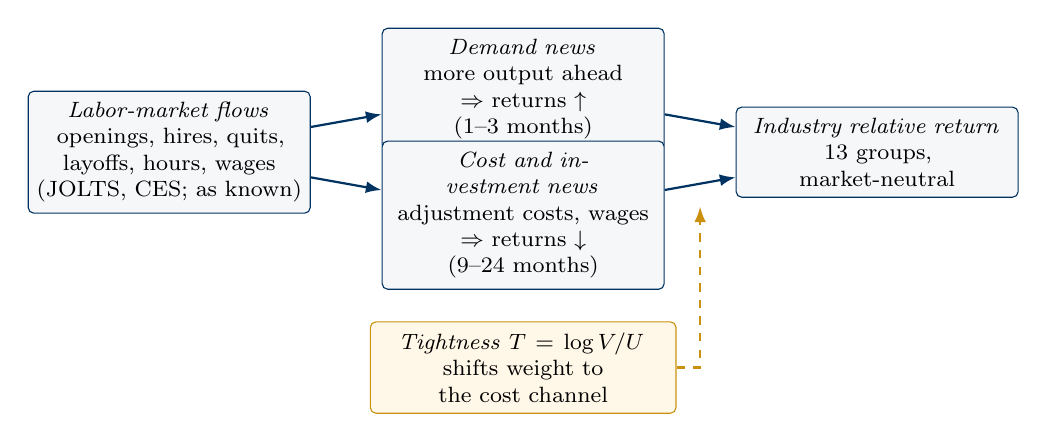
\begin{tikzpicture}[
  node distance=5mm and 9mm,
  box/.style={draw=bblue,rounded corners=2pt,fill=bblue!4,align=center,font=\footnotesize,inner sep=4pt,text width=3.3cm},
  mod/.style={draw=bgold!80!black,rounded corners=2pt,fill=bgold!10,align=center,font=\footnotesize,inner sep=4pt,text width=3.6cm},
  arr/.style={-{Latex[length=2mm]},thick,bblue}]
  \node[box] (data) {\emph{Labor-market flows}\\openings, hires, quits,\\layoffs, hours, wages\\(JOLTS, CES; as known)};
  \node[box,right=of data,yshift=8mm] (dem) {\emph{Demand news}\\more output ahead\\$\Rightarrow$ returns $\uparrow$ (1--3 months)};
  \node[box,right=of data,yshift=-8mm] (cost) {\emph{Cost and investment news}\\adjustment costs, wages\\$\Rightarrow$ returns $\downarrow$ (9--24 months)};
  \node[box,right=of dem,yshift=-8mm] (ret) {\emph{Industry relative return}\\13 groups, market-neutral};
  \node[mod,below=4mm of cost] (tight) {\emph{Tightness} $T=\log V/U$\\shifts weight to the cost channel};
  \draw[arr] (data) -- (dem); \draw[arr] (data) -- (cost);
  \draw[arr] (dem) -- (ret); \draw[arr] (cost) -- (ret);
  \draw[-{Latex[length=2mm]},thick,bgold!80!black,dashed] (tight.east) -| ($(cost.east)!0.5!(ret.south west)$);
\end{tikzpicture}
\caption{Labor flows carry two kinds of industry news with opposite sign and different horizons; tightness should change which one dominates. \hfill\tagc}
\label{fig:thesis}
\end{figure}

\Cref{tab:hyp} lists each signal, the sign we preregistered and the mechanism behind it. The last column, added after the fact, shows what the data say.

\begin{table}[H]
\centering\small
\begin{threeparttable}
\caption{Signals, preregistered signs and what the data say. \hfill\tagc\ (design) / \tagp\ (last column)}
\label{tab:hyp}
\begin{tabularx}{\textwidth}{@{}l Y c Y r@{}}
\toprule
Signal & Definition (group $g$, month $t$) & Prior & Mechanism & IC, $h{=}1$ \\
\midrule
F1 openings & 12-month change in 3-month average openings rate & $+$ & demand news & $-0.005$ \\ % src: claim D02
F2 hires    & same, hires rate & $+$ & demand news; investment channel $-$ at long horizon & $+0.013$ \\ % src: claim D02
F3 quits    & same, quits rate & none & worker bargaining power & $+0.009$ \\ % src: claim D02
F4 layoffs  & same, layoffs rate & $-$ & negative demand shock & $+0.028$ \\ % src: claim D02
F5 hours    & 12-month log change, average weekly hours & $+$ & intensive-margin demand & $-0.010$ \\ % src: claim D02
W wages     & 12-month log change, average hourly earnings & dropped & cost pressure ($-$) vs.\ labor risk premium ($+$) & $+0.039$ \\ % src: claim D01
\bottomrule
\end{tabularx}
\begin{tablenotes}\footnotesize
\item IC (information coefficient) is the average monthly Spearman correlation between the signal and the next month's industry relative return, May 2004 to August 2026, revised data with publication lags; only W has $|t|>2$ ($t=2.50$). % src: claim D01
The preregistered fixed rule A0 used $z(\text{F1})+z(\text{F2})-z(\text{F4})+z(\text{F5})$; the data reject the signs of F4 and F5. % src: claim D03
\end{tablenotes}
\end{threeparttable}
\end{table}

\subsection{Data}

\begin{table}[H]
\centering\small
\caption{Data sources (all free; links in \cref{app:data}). \hfill\tagc}
\label{tab:data}
\begin{tabularx}{\textwidth}{@{}l Y c c Y@{}}
\toprule
Source & Series & Freq. & Known at $t$ & Vintage handling in the frozen study \\
\midrule
BLS JOLTS & openings, hires, quits, layoffs rates; 13 industries; not seasonally adjusted & M & $t-2$ & ALFRED vintages: the value known on each decision date \\
BLS CES   & average weekly hours and hourly earnings, production and nonsupervisory workers & M & $t-1$ & as above \\
FRED      & total openings (JTSJOL) and unemployed (UNEMPLOY) for $T_t$ & M & $t-2$ & as above \\
Ken French & 49 value-weighted industry portfolios $\to$ 13 groups; five factors and momentum & M & $t$ & CRSP build 202608 \\
\bottomrule
\end{tabularx}
\end{table}

\paragraph{Universe} The 49 French industries are mapped to the 13 JOLTS/CES industry groups and value-weighted within each group (\cref{app:mapping}). The mapping is coarse: labor data describe every establishment in an industry, while returns describe listed firms. Durable manufacturing is 60\% semiconductors by market capitalisation and nondurable manufacturing 60\% pharmaceuticals. % src: claim S03

\paragraph{Point-in-time data} Labor data are revised after first release, so today's values leak information. The frozen study rebuilt every series as it stood on each decision date from ALFRED vintages (78 series) and kept three alternatives: first release, fully revised, and revised with fixed publication lags. The primary result barely depends on the choice: A3's test Sharpe is $-0.58$ as known, $-0.52$ on first releases, $-0.56$ revised and $-0.53$ with fixed lags. % src: claim C20
Our post-hoc work (\cref{sec:survives}) uses revised data with fixed lags, which reproduces the frozen fixed-lag signal with a pooled correlation of 0.998, % src: claim S01
but as-known data pick the same top-three groups in only 42\% of months, % src: claim S02
so post-hoc holdings, though not the conclusions, would have differed in real time.

\paragraph{Sample} Research (signal design and model selection): May 2004 to September 2014, 125 months. Test, opened once: November 2014 to August 2026, 142 months. % src: claim S05
\Cref{fig:timeline} shows why the tightness hypothesis could not be learned: $V/U$ never exceeded 1 in the research period and exceeded it in 75 test months. % src: claim D06

\begin{figure}[H]
\centering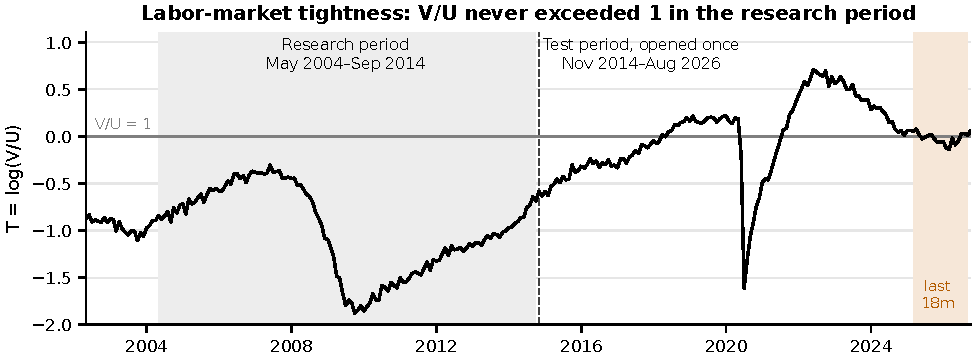
\includegraphics[width=0.92\linewidth]{figures/fig_timeline.pdf}
\caption{Tightness never exceeded $V/U=1$ in the research period, so a moderator learned there is extrapolated throughout the test. \hfill\tagp}
\label{fig:timeline}
\end{figure}

\subsection{Implementation}

\paragraph{Signals} For a labor series $x_{g,t}$ in group $g$, let $\bar x_{g,t}=\tfrac13(x_{g,t}+x_{g,t-1}+x_{g,t-2})$. With publication lag $\ell$ (2 months for JOLTS, 1 for CES),
\begin{equation}
F_{g,t}=\bar x_{g,t-\ell}-\bar x_{g,t-\ell-12}\qquad\text{(log differences for hours and earnings).}
\end{equation}
Each signal is divided by its own expanding-window standard deviation (at least 24 months), z-scored across the 13 groups and winsorised at $\pm3$, giving $z^{(k)}_{g,t}$. Year-over-year differences remove seasonality, which lets us use the not-seasonally-adjusted series that exist for every industry.

\paragraph{Models} \Cref{tab:models} lists the five preregistered strategies. The learned ones are ridge regressions of next-month relative return on the signals,
\begin{equation}
\hat\beta_t=\arg\min_\beta \sum_{s<t}\sum_g\big(r^{\mathrm{rel}}_{g,s+1}-z_{g,s}^{\top}\beta\big)^2+\alpha\lVert\beta\rVert^2,
\end{equation}
re-estimated each month on an expanding window, with $\alpha$ chosen once by blocked cross-validation inside the research period over a grid from 0.01 to 1000. Cross-validation chose 1000, the top of the grid, for every model: % src: claim C18
the data were asking for no forecast at all.

\begin{table}[H]
\centering\small
\caption{Preregistered strategies (legend for the codes used below). \hfill\tagc}
\label{tab:models}
\begin{tabularx}{\textwidth}{@{}l X@{}}
\toprule
A0 & Fixed rule, no estimation: $S_{g,t}=\tfrac14\big(z^{(1)}+z^{(2)}-z^{(4)}+z^{(5)}\big)$. \\
A1 & Ridge on F1--F5. \\
A1-T & A1 plus each signal interacted with tightness $T$. \\
A3 & A1 plus features proposed by \emph{independent} LLM agents (\cref{sec:ai}); the primary, chosen on research data. \\
A4 & A1 plus features proposed by \emph{communicating} LLM agents. \\
\bottomrule
\end{tabularx}
\end{table}

\paragraph{Portfolio, risk model and costs} Each month the score $s_{m,g}$ known at the end of month $m-1$ is converted to a dollar-neutral tranche, long the three highest-ranked groups and short the three lowest; the book averages the last three tranches, is hedged to zero market beta, scaled to a 10\% ex-ante volatility and capped at a gross exposure of 2, and pays 10\,bp per unit of industry turnover plus 2\,bp on the hedge:
% Score-to-weight mapping of the frozen study's backtest (study1_preregistered/outputs/follow_the_workers/data.py::backtest).
% Written by analysis/run.ipynb. Parameters: analysis/params.py PORTFOLIO (checked equal to the frozen params in Gate 1).
\begin{align}
\tau_{m,g} &= \begin{cases} +\tfrac13 & g \in \text{top 3 of } s_{m,\cdot}\\ -\tfrac13 & g \in \text{bottom 3 of } s_{m,\cdot}\\ 0 & \text{otherwise}\end{cases}
  \qquad b_{m} = \frac{1}{H}\sum_{j=0}^{H-1} \tau_{m-j}, \quad H=3, \label{eq:tranche}\\
h_{m} &= -\sum_{g} b_{m,g}\,\hat\beta_{m,g}, \qquad x_m = (b_{m,1},\dots,b_{m,13},\,h_m), \label{eq:hedge}\\
k_m &= \min\!\left(\frac{0.10}{\sqrt{12\,x_m^{\top}\hat\Sigma_m x_m}},\ \frac{2}{\lVert x_m\rVert_1}\right), \qquad w_m = k_m\,x_m, \label{eq:scale}\\
r^{\mathrm{net}}_{m} &= \sum_{g} w_{m,g}\, r^{e}_{m,g} + w_{m,M}\,\mathrm{MKT}_m
  - c\sum_{g}\lvert w_{m,g}-\tilde w_{m,g}\rvert - c_h\,\lvert w_{m,M}-\tilde w_{m,M}\rvert. \label{eq:net}
\end{align}
where $s_{m,g}$ is the score of group $g$ known at the end of month $m-1$, $\hat\beta_{m,g}$ and the Ledoit--Wolf covariance
$\hat\Sigma_m$ (13 groups plus the market) use the 60 months ending in $m-2$ (at least 36), $r^{e}_{m,g}$ is the group's excess
return, $\tilde w$ are the previous weights after drift, $c=10$\,bp and $c_h=2$\,bp.

In the test the cap, not the volatility target, bound in 87\% of A3's months, so realised volatility ran at 7.8\% against the 10\% target. % src: claim D13

\begin{keybox}[How we kept the test honest]
\begin{itemize}[leftmargin=*]
  \item Every input as it was known on the decision date (ALFRED vintages); the primary result is unchanged under four data vintages. % src: claim C20
  \item Signals, models, the primary strategy and five pass/fail gates (G1 timing, G2 prediction, G3 incremental alpha, G4 robustness, G5 implementability) were fixed and hashed before any test data were touched; the test period was opened exactly once.
  \item Every result reported whatever its sign: a circular-shift placebo with full refits, drop-one-industry checks, Holm-adjusted bootstrap comparisons and a deflated Sharpe ratio \citep{BaileyLopezdePrado2014}.
  \item Anything decided after seeing test results is labelled \tagp\ and was itself written to a file and hashed before it ran; the live out-of-sample book is labelled \tagf. \todo{Alex: confirm the freeze hashes and the single opening against FREEZE.json and evaluation\_started.json}
\end{itemize}
\end{keybox}

\paragraph{AI-assisted signal search}\label{sec:ai} We asked large language model (LLM) agents to propose new labor features from six anonymised variables using a restricted formula grammar. Two arms of three agents each, \emph{independent} versus \emph{islands} that exchange short migration reports, ran three repetitions, for 108 proposals per study (\cref{fig:agents}). Selection was mechanical (research $t\ge1.5$, same sign in both halves, low correlation, at most three per arm). An LLM judge, audited by a human, scored whether ideas spread between agents. The agents were Claude Sonnet~5.5 in the confirmatory study and Claude Opus~5.5 in an exploratory follow-up run after the test had been seen (\cref{app:opus}).

\begin{figure}[H]
\centering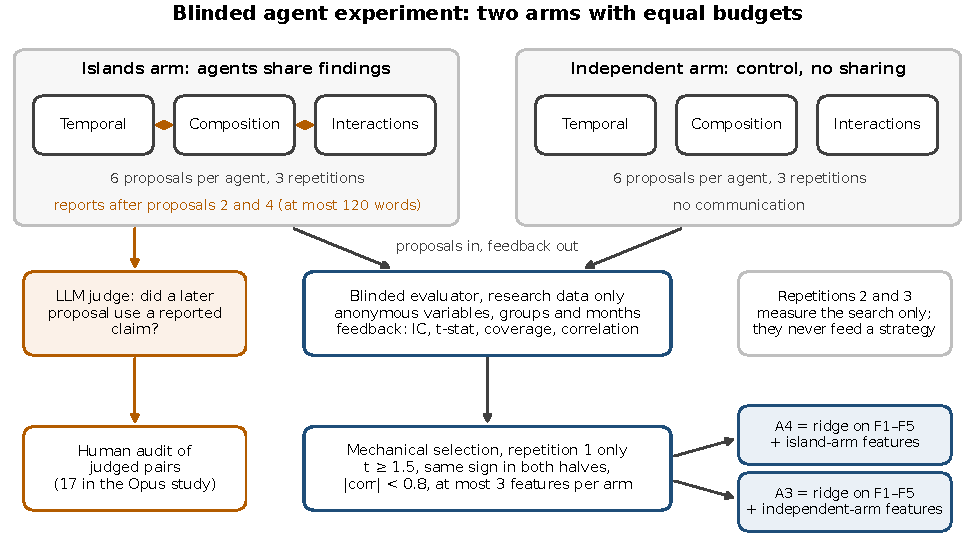
\includegraphics[width=0.88\linewidth]{figures/fig_agents.pdf}
\caption{Two arms with equal budgets, a blinded evaluator, mechanical selection and a human-audited LLM judge. \hfill\tagc}
\label{fig:agents}
\end{figure}

\paragraph{Claude as research assistant} We used Claude (Anthropic) at four points of the build: auditing sources and code (P1), proposing signals as blinded agents (P2), judging whether ideas spread (P3) and red-teaming the robustness plan (P4). We used it again to review the finished study (P5) and to run this iteration (P6). Three of the prompts, verbatim, are below; outputs and our evaluation are in \cref{sec:claude}, transcripts in \cref{app:transcripts}.

\begin{promptbox}{Prompt P1: source and code review}
Find mapping errors, timestamp or look-ahead errors, and code bugs in the material below. For each problem, give the exact line or row, why it is wrong, and a test that would confirm it. Do not report style issues. [followed by the series manifest, the industry crosswalk and the as-of code]
\end{promptbox}
\begin{promptbox}{Prompt P2: blinded signal-search agent (system prompt, opening)}
You are a quantitative researcher. You will propose one feature per turn to predict which of 13 anonymous groups (G01 to G13) will have higher returns next month relative to the others. You see only the variable dictionary below, the allowed operations, and summary statistics of your previous submissions. You do not know what the groups, variables or time periods are. Do not guess them and do not use knowledge about any real industry, company or date. [variable dictionary, grammar and JSON format follow]
\end{promptbox}
\begin{promptbox}{Prompt P4: robustness red team}
Give 10 distinct reasons these results could be spurious, ranked by likelihood. For each, name a test that can be run with this data and the result that would make us say "do not implement". [followed by the research-period result tables, without dates or names]
\end{promptbox}

% =====================================================================
\section{What did we learn?}

\Cref{tab:sealed} reports the one-time test. No strategy made money; the primary lost 4.6\% a year with a 41\% drawdown % src: claim C02
and failed four of the five gates. % src: claim C07
Costs are not the explanation: A3 paid 1.1\% a year in trading costs against a gross loss of 3.5\%, % src: claim C15
and it would lose money even if industry trading were free (break-even cost $-32$\,bp). % src: claim C06

\begin{table}[H]
\centering\small
\begin{threeparttable}
\caption{Preregistered strategies: research versus the one-time test. \hfill\tagc}
\label{tab:sealed}
\begin{tabular}{@{}lrrrrr@{}}
\toprule
 & Research & \multicolumn{4}{c}{Test, Nov 2014--Aug 2026 (142 months)}\\
\cmidrule(l){3-6}
Strategy & Sharpe & Sharpe & Net return & Volatility & Max drawdown \\
\midrule
A0 fixed rule   & $-0.44$ & $-0.36$ & $-3.5\%$ & $9.7\%$ & $-40.3\%$ \\ % src: claims C09, C08; d4_test_performance.csv
A1 ridge        & $-0.54$ & $-0.51$ & $-4.0\%$ & $7.9\%$ & $-37.7\%$ \\ % src: claims C09, C08; d4_test_performance.csv
A1-T tightness  & $-0.55$ & $-0.59$ & \prov{$-4.9\%$} & \prov{$8.2\%$} & \prov{$-36.3\%$} \\ % src: claims C09, C08; results.json variants.ASOF.A1-T (not in register)
A3 primary      & $-0.13$ & $-0.58$ & $-4.6\%$ & $7.8\%$ & $-41.1\%$ \\ % src: claims C09, C01, C02
A4 islands      & $-0.18$ & $-0.79$ & $-6.1\%$ & $7.8\%$ & $-53.3\%$ \\ % src: claims C09, C08; d4_test_performance.csv
\bottomrule
\end{tabular}
\begin{tablenotes}\footnotesize
\item Annualised, net of costs, as-known data; research Sharpe over the 88 months in which every model had a forecast. % src: claim C09
Primary: IC $-0.021$ ($t=-1.08$), placebo $p=0.72$, factor alpha $-0.38\%$ a month ($t=-1.86$), Sharpe $-0.79$ at 25\,bp costs; gate G1 passed, G2--G5 failed. % src: claims C03, C05, C04, C04b, C12, C07
Every Holm-adjusted pairwise comparison had adjusted $p=1.0$. % src: claim C16
\end{tablenotes}
\end{threeparttable}
\end{table}

\subsection{Style and risk exposures}
The labor books are quality and growth tilts rather than bets on labor news. Regressing monthly returns on the Fama--French five factors, momentum and an industry-momentum factor (\cref{fig:loadings}, appendix), the primary loads on profitability (RMW $+0.19$, $t=2.2$) and against value (HML $-0.15$, $t=-2.0$), with no market or momentum exposure and an alpha of $-0.38\%$ a month ($t=-1.86$). % src: claims C13, C04, C04b
That is plausible: industries adding workers and hours are the profitable, growing ones, so a long-hiring book buys profitability and sells value. The post-hoc wage-growth book tilts the same way but harder, against value (HML $-0.43$, $t=-4.4$) and towards momentum ($+0.22$, $t=3.3$), % src: claim V11
while the 12-month hiring-reversal book loads the other way, against profitability (RMW $-0.36$, $t=-4.45$). % src: claim R6b
Only the fixed rule A0 carries a visible industry-momentum loading ($+0.22$, $t=1.9$). % src: claim C14

\subsection{Time patterns of performance}
\Cref{tab:windows} covers the course windows. For the confirmatory primary, ``post-2010'' and the test nearly coincide, because the test starts in November 2014; the ``full'' window mixes the research years, in which the model was chosen, with the test, and is descriptive. The primary's one bright spot, $+0.85$ over the last 18 months, rests on an IC $t$ of 0.44 and does not survive the whole test. % src: claim C10; results.json windows.A3.last_18.IC.t
The post-hoc books show the opposite pattern: wage growth did well until 2024 and lost heavily in the last 18 months ($-1.71$), % src: claim V_V2a_SR
while the 12-month hiring book is the only one positive in every window (cumulative paths in \cref{fig:cumulative}, appendix). % src: claim V_V2d_SR

\begin{table}[H]
\centering\small
\begin{threeparttable}
\caption{Net Sharpe ratio by window. \hfill\tagc\ (A3) / \tagp\ (V2a, V2d)}
\label{tab:windows}
\begin{tabular}{@{}lrrrrr@{}}
\toprule
 & Research & Test & Full sample & Post-2010 & Last 18 months \\
Window (returns) & 2004--14 & 2014--26 & 2004--26 & 2010--26 & 2025-03--2026-08 \\
\midrule
A3 primary (confirmatory)      & $-0.13$ & $-0.58$ & $-0.44$ & $-0.62$ & $+0.85$ \\ % src: claims C09, C01, C11, C10
V2a wage growth (post-hoc)     & $+0.09$ & $+0.16$ & $+0.15$ & $+0.12$ & $-1.71$ \\ % src: claim V_V2a_SR
V2d $-$(hires+quits), 12m (post-hoc) & $+0.50$ & $+0.29$ & $+0.35$ & $+0.30$ & $+0.29$ \\ % src: claim V_V2d_SR
\bottomrule
\end{tabular}
\begin{tablenotes}\footnotesize
\item A3's research and full-sample figures use the 88 months with a forecast (from June 2007) and are descriptive; V2a and V2d use revised data with fixed lags over 125, 142, 268, 200 and 18 months. % src: claims C09, S05
\end{tablenotes}
\end{threeparttable}
\end{table}

\subsection{Robustness and limits}\label{sec:robust}

\paragraph{What the universe allows} By the fundamental law of active management, the information ratio (IR) of a book is roughly $\mathrm{IC}\times\sqrt{\mathrm{BR}}\times\mathrm{TC}$, with BR the number of independent bets a year and TC the transfer coefficient between the signal and the weights actually held. With 13 groups a monthly book has BR of at most 156 and a 12-month book 13, so a monthly IC of 0.05 caps the IR near 0.6 and a 12-month IC of 0.10 near 0.35. In the test, A3's IC of $-0.021$ and TC of 0.80 imply $-0.21$ against a realised $-0.58$; V2a's IC of $+0.049$ implies $+0.56$ against a realised $+0.16$; V2d's 12-month IC of $+0.096$ with a TC of 0.48 implies $+0.17$ against a realised $+0.29$. % src: claim R11a
A modest Sharpe ratio is the ceiling for this universe, and the preregistered overlay (hedge, volatility target, binding cap, 0.9 turnover a month) % src: claim C21
cost the monthly books most of what their IC allowed.

\paragraph{Why the preregistered design failed} Four reasons, each visible in the data (figures in \cref{app:results}).
\begin{enumerate}[leftmargin=*]
  \item \emph{Wrong signs.} Layoffs carry a positive IC in both periods and hours a negative one, the opposite of the signs A0 imposed (\cref{tab:hyp}). % src: claim D03
  Wage growth, which the blueprint included and the build dropped with the price series it was paired with, is the only signal with a positive IC in both periods ($+0.029$ research, $+0.049$ test). % src: claim D01
  \item \emph{Wrong horizon.} At one month no hiring signal predicts returns; at twelve months hires ($-0.062$, $t=-2.1$) and quits ($-0.065$, $t=-1.7$) carry the negative sign the investment channel predicts. % src: claim D04
  We traded the demand channel at a horizon where only the cost channel shows up.
  \item \emph{An untestable moderator.} Tightness terciles were set on an expanding window; because the research years never saw a tight market, 133 of 142 test months fell in the ``high'' tercile. % src: claim D06
  A split on whether $T$ rose or fell over 12 months (93/32 research months, 88/54 test) would have been testable. % src: claim D07
  \item \emph{Fragile agent features.} The two features selected for the primary were gated on the ``low tightness'' regime and were active in 3 of 142 test months. % src: claim D12
  Every feature that passed research failed the test (4 of 4 Sonnet, 6 of 6 Opus). % src: claim C19
\end{enumerate}
Losses were concentrated: health care cost the primary 26 points of cumulative return, construction 19 and finance 16, against 13 points of trading costs. % src: claim D09

\paragraph{What survives, and how much}\label{sec:survives} After the test was opened we froze four variants in a hashed file (\path{analysis/v2_spec.md}) with a reading rule, ran each once and report all four (\cref{tab:v2}). None meets the rule, which required a positive Sharpe at 25\,bp, IC $t\ge2$, alpha $t\ge2$, positive IC in both test halves, placebo $p<0.05$ and a deflated Sharpe ratio (DSR) above 0.95. % src: claim V07
The declared headline, a wage-growth rank (V2a), has the right IC ($+0.049$, $t=2.04$, placebo $p=0.02$) but no alpha ($t=0.29$) and a DSR of 0.02: % src: claim V01
a value and momentum tilt that happened to work. Adding momentum (V2c) raises the Sharpe to $+0.35$ because momentum supplies the return, and the learned-sign composite (V2b) is negative. % src: claims V_V2c_SR, V05, V_V2b_SR
The variant that answers the thesis is V2d: $-\tfrac12(z(\text{F2})+z(\text{F3}))$, short the industries that hire and lose workers fastest, held twelve months. Its score has no one-month IC ($-0.020$, $t=-0.87$) and a positive IC from 9 to 24 months, peaking at 12 ($+0.096$, $t=2.43$; \cref{fig:horizon_profile}). % src: claim R2a
Its alpha is $+0.26\%$ a month ($t=1.48$ in the test, $1.92$ over the full sample, 12 HAC lags). % src: claims R6a, R6a2

\begin{table}[H]
\centering\footnotesize
\caption{Post-hoc variants frozen in \texttt{analysis/v2\_spec.md}: net Sharpe by window and test statistics at 10\,bp; DSR counts 112 looks. \hfill\tagp}
\label{tab:v2}
% POST-HOC | source: analysis/output/tables/v2_results.csv (generated by analysis/run.ipynb)
\begin{tabular}{lrrrrrrrrr}
\toprule
Variant & Research & Test & Full & Post-2010 & Last 18m & Test IC (t) & Alpha t & Placebo p & DSR \\
\midrule
V2a & +0.09 & +0.16 & +0.15 & +0.12 & $-$1.71 & +0.049 (+2.04) & +0.29 & 0.02 & 0.02 \\
V2b & $-$0.06 & $-$0.15 & $-$0.11 & $-$0.16 & $-$1.34 & +0.042 (+1.65) & $-$0.84 & 0.05 & 0.00 \\
V2c & +0.27 & +0.35 & +0.32 & +0.24 & $-$0.78 & +0.032 (+1.21) & +1.36 & 0.26 & 0.09 \\
V2d & +0.50 & +0.29 & +0.35 & +0.30 & +0.29 & $-$0.020 ($-$0.87) & +1.37 & 0.85 & 0.06 \\
\bottomrule
\end{tabular}

\end{table}

\begin{figure}[H]
\centering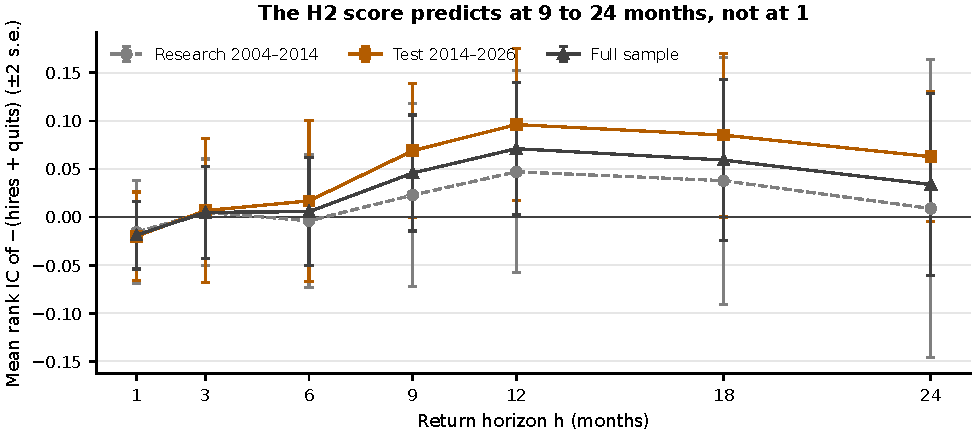
\includegraphics[width=0.86\linewidth]{figures/fig_horizon_profile.pdf}
\caption{The thesis result: the hiring score has no one-month IC and a positive IC from 9 to 24 months, peaking at 12 (test $+0.096$, $t=2.43$). \hfill\tagp}
\label{fig:horizon_profile}
\end{figure}

\paragraph{How robust is V2d?} We froze a second file (\path{analysis/v3_spec.md}) with eleven checks and a reading rule, raised the look count to 132 and ran it once. V2d is not carried by one component (hires alone $+0.19$, quits alone $+0.16$), % src: claim R1a
by one holding period (9 months $+0.14$, 12 $+0.29$, 18 $+0.30$), % src: claim R3a
by costs (break-even 68\,bp; $+0.22$ at 25\,bp, $+0.09$ at 50) % src: claim R5a
or by one industry (dropping any one leaves the test Sharpe between $+0.18$ and $+0.48$). % src: claim R7a
It fails one pre-declared condition: it lost money in the first half of the test ($-0.21$) and made it in the second ($+0.64$), % src: claim R4a
although its 12-month IC was positive in both halves ($+0.097$, $+0.095$). % src: claim R4c
A block-bootstrap 90\% interval for the test Sharpe, $[-0.07,+0.65]$, includes zero; the full-sample interval, $[+0.05,+0.64]$, does not. % src: claim R9a
After 132 looks the DSR is 0.05 in the test and 0.16 over the full sample. % src: claim R12
We read this as a hypothesis with the right economics and too little data, not as alpha. One pattern is recorded without a claim: V2d earned its return when tightness was falling or $V/U$ exceeded 1 and nothing while the market tightened, on 54 to 88 months per cell (\cref{fig:v2d_tightness}). % src: claim R8a

\paragraph{Live forward test} On 3 October 2026 we froze a forward specification (hash \texttt{735a8ffa}, amended by \texttt{c76cde86} after a data-release check stopped the first run) and built the Q4 2026 books for the 30 September decision from data published by 29 September. % src: claims F08, F05
Each book has three longs and three shorts, a 60-month beta hedge in SPY, and is held to 31 December. V2a is long construction, durable manufacturing and information and short mining, health care and accommodation; % src: claim F01
V2d is long finance, real estate and accommodation and short mining, durable manufacturing and retail. % src: claim F02
V2c's tradable book has four legs, because its long durable-manufacturing and short professional-services positions both map to the industrials ETF and cancel. % src: claim F04
V2c and V2d were added after the historical v2 results had been seen and before any Q4 return beyond 1--2 October existed; we say so because it is a selection step. One quarter has almost no power: a Q4 return anywhere between $-10\%$ and $+10\%$ is consistent with no skill (\cref{app:forward}).

\paragraph{Limits} With 142 test months only a Sharpe near 0.6 reaches $t\approx2$, so a null does not rule out a smaller effect, and none of our post-hoc Sharpe ratios is distinguishable from zero after deflation. % src: claim C22
The 49-to-13 mapping dilutes the labor signal; the one near-positive result in the Opus follow-up came from a single long position in a group that is 60\% semiconductors (\cref{app:opus}). % src: claims X04, S03
All post-hoc numbers use revised data with fixed lags; the as-known rerun was not run for lack of an API key. % src: claim R10
NAICS-based stock baskets built from CRSP, which would raise breadth and sharpen the mapping, are the follow-up we would run next.

\subsection{Claude evaluation}\label{sec:claude}

\Cref{tab:claude} records every Claude interaction. The models are taken from the call logs: Sonnet~5.5 at medium effort for the 607 calls of the confirmatory study, Opus~5.5 at extra-high effort for the 905 calls of the follow-up. \todo{Alex: exact name and vendor of the engineering assistant that wrote the pipeline code (``6 astra''); it is not documented in the repository}

\begin{table}[H]
\centering\scriptsize\setlength{\tabcolsep}{3pt}
\caption{Claude as research assistant: six interactions. \hfill\tagc\ (P1--P4) / \tagp\ (P5--P6)}
\label{tab:claude}
\begin{tabularx}{\textwidth}{@{}l Y Y Y Y Y@{}}
\toprule
 & What we asked & What it got right & What it got wrong & What we changed & Our critique \\
\midrule
P1 audit & Find mapping, timing and code errors in the manifest, crosswalk and as-of code & 25 numbered findings; the shared CES series for groups 9 and 10 & Several alleged look-ahead errors were not errors; no numeric change resulted & Mapping metadata relabelled; no basket changed & \todo{critique: Alex} \\
P2 agents & Propose features from six anonymous variables within a grammar (two arms, six turns, three repetitions) & Valid grammar in 98 of 108 proposals (106 for Opus); both studies rediscovered wage growth from the anonymised variable % src: claims A01, A02
 & The best research $t$-statistics came from regime gates active in 3 test months; every selected feature failed the test % src: claims D12, C19
 & Selection stayed mechanical; v2 restores wage growth as a public, ungated signal & \todo{critique: Elouan} \\
P3 judge & Write migration reports; judge whether later proposals used a reported claim & Opus: 15 of 18 reports admitted, 84 of 88 labels usable % src: claim A02
 & Sonnet: 28 of 36 judge outputs were not valid JSON; the judge said yes 10 times where the human said 3, all 7 disagreements judge-yes % src: claims A01, A02, A03
 & Judge labels reported as associations next to the human labels & \todo{critique: Al Yazid} \\
P4 red team & Ten reasons the research results could be spurious, each with a test & Ranked, specific; called ``do not implement'' from research tables before the seal opened & Quoted p-values it had not computed; proposed unregistered thresholds & No new test adopted; each concern was already covered & \todo{critique: Romain} \\
P5 review & Read the frozen study and say what is wrong with it (Opus, Claude Code) & Wrong signs, dropped wage signal, 12-month hiring sign, 3-month agent features, one-bin tightness split & Guessed the engineering assistant was OpenAI Codex; a momentum definition that included the latest month; wage ICs with a non-frozen start date & Momentum redefined; wage ICs recomputed; the guess withdrawn & \todo{critique: Piero} \\
P6 iteration & Rebuild the analysis, freeze and run v2/v3, build the forward book, draft this report & Reproduced the sealed returns to $10^{-16}$; froze every spec before running; reported every variant; stopped at a failed gate & Assumed August JOLTS would not be out by 29 September; it was, so its own check stopped the run & Amendment 001, disclosed; run logs that make every result byte-reproducible & \todo{critique: Alex} \\
\bottomrule
\end{tabularx}
\end{table}

\paragraph{Agents: capability is not alpha} Compared with Sonnet, Opus produced more valid proposals (106 of 108 against 98), more admitted migration reports (15 of 18 against 7) and far more usable judge labels (84 of 88 against 8 of 36), % src: claims A01, A02
and more of its features passed the research filter (7 against 4), % src: claim X05
yet none survived the test in either study. % src: claim C19
Communication raised research search scores for one model (best IC 0.136 against 0.059 for the independent arm) and lowered them for the other (0.049 against 0.083); neither gap exceeded the spread across repetitions. % src: claim A05
The judge's over-attribution means that measured ``idea uptake'' overstates how much the agents built on each other.

\paragraph{Reflection} \prov{draft} Claude was most useful where the task had a checkable answer: reproducing numbers, auditing code and timing, listing failure modes. It was least useful where the task needed judgement about evidence: features that were artefacts of a regime gate, a judge that over-attributed, a red team that invented statistics. What protected us was mechanics, not prompts: blinding, a fixed evaluator, hashed specifications and a test opened once. \todo{Al Yazid: rewrite in the team's words; remove the draft mark}

% =====================================================================
\bibliographystyle{plainnat}
\bibliography{refs}

% =====================================================================
\clearpage
\appendix
\section{Claude interaction transcripts}\label{app:transcripts}
Paths are relative to \path{230ga-follow-the-workers/outputs/follow_the_workers/} unless stated; the Opus follow-up has the same files under \path{follow_the_workers_opus55_xhigh/}.
\begin{itemize}
  \item P1: prompt \path{outputs/p1_request.json} (the instruction in \cref{sec:ai} followed by the manifest, crosswalk and as-of code); response \path{outputs/p1_response.md}; dispositions \path{outputs/p1_review.md}. \todo{Alex: add the disposition counts from p1\_review.md}
  \item P2: system and turn prompts in \path{params.py} (\texttt{SYSTEM\_PROMPT}, \texttt{TURN\_PROMPT}); every call with its raw response in \path{outputs/agents/log.jsonl}; proposals in \path{outputs/candidates.csv}; selected features decoded in \path{analysis/output/tables/d7_selected_features.csv}.
  \item P3: migration reports in \path{outputs/agents/migrations.json}; the judge prompt in \path{agents.py}, function \path{trace_migrations}; judgments in \path{outputs/agents/migration_judgments.json}; the human audit in \path{outputs/human_review_submission.md}.
  \item P4: prompt \path{outputs/p4_request.json}; response \path{outputs/p4_response.md}; dispositions \path{outputs/p4_review.md}.
  \item P5: the review and its output, \path{FINDINGS_AND_PROPOSAL.md}, with the numbers in \path{analysis/output/diagnostics.md}.
  \item P6: the task files \path{ITERATION_PROMPT.md} and \path{OVERNIGHT_PROMPT.md}; the rules in \path{CLAUDE.md}; outputs in \path{analysis/run.ipynb}, \path{analysis/output/}, \path{results/} and this report.
\end{itemize}

\section{Data links}\label{app:data}
\begin{itemize}
  \item Ken French Data Library: \url{https://mba.tuck.dartmouth.edu/pages/faculty/ken.french/data_library.html} (49 industry portfolios, five factors, momentum; CRSP build 202608).
  \item JOLTS by industry, not seasonally adjusted: FRED series \texttt{JTU<code>JOR/HIR/QUR/LDR}, for example \url{https://fred.stlouisfed.org/series/JTU2300HIR}; codes 110099, 2300, 3200, 3400, 4200, 4400, 480099, 5100, 5200, 5300, 540099, 6200, 7200.
  \item CES hours and earnings: \texttt{CEU<code>07} and \texttt{CEU<code>08} (construction earnings \texttt{CES2000000008}); codes 10000000, 20000000, 31000000, 32000000, 41420000, 42000000, 43000000, 50000000, 55000000, 60000000, 65000000, 70000000.
  \item Tightness: \texttt{JTSJOL} and \texttt{UNEMPLOY}. Vintages: \url{https://alfred.stlouisfed.org/}.
  \item ETF proxies and their caveats: \path{analysis/forward/etf_proxies.csv}. \todo{Elouan: check every link and add access dates}
\end{itemize}

\section{Industry mapping}\label{app:mapping}
\begin{table}[H]
\centering\footnotesize
\caption{The 13 groups: JOLTS code, Ken French members and the largest member's share of August 2026 market capitalisation. \hfill\tagc}
\begin{tabularx}{\textwidth}{@{}l l X l@{}}
\toprule
Group & JOLTS & Ken French industries & Largest member \\
\midrule
Mining and logging & 110099 & Gold, Mines, Coal, Oil & Oil 79\% \\ % src: analysis/forward/etf_proxies.csv group_composition_aug2026
Construction & 2300 & Cnstr & 100\% \\
Durable manufacturing & 3200 & Toys, BldMt, Steel, FabPr, Mach, ElcEq, Autos, Aero, Ships, Guns, Hardw, Chips, LabEq, MedEq & Chips 60\% \\ % src: claim S03
Nondurable manufacturing & 3400 & Food, Soda, Beer, Smoke, Hshld, Clths, Drugs, Chems, Rubbr, Txtls, Paper & Drugs 60\% \\ % src: claim S03
Wholesale & 4200 & Whlsl & 100\% \\
Retail & 4400 & Rtail & 100\% \\
Transport and utilities & 480099 & Trans, Util & Util 61\% \\ % src: etf_proxies.csv
Information & 5100 & Telcm & 100\% \\
Finance and insurance & 5200 & Banks, Insur, Fin & Banks 51\% \\ % src: etf_proxies.csv
Real estate & 5300 & RlEst & 100\% \\
Professional and business services & 540099 & BusSv & 100\% \\
Health care & 6200 & Hlth & 100\% \\
Accommodation and food & 7200 & Meals & 100\% \\
\bottomrule
\end{tabularx}
\end{table}
Groups 9 and 10 share one CES series, and groups 7, 12 and 13 use broader CES supersectors, so the effective cross-sectional width is closer to 8 or 9 than 13.

\section{Full results and figures}\label{app:results}
\paragraph{Data vintages} A3 test Sharpe: as-known $-0.58$, first release $-0.52$, revised $-0.56$, fixed lags $-0.53$; IC $-0.021$, $-0.040$, $-0.026$, $-0.021$. % src: claim C20
\paragraph{Cost sensitivity} A3 Sharpe $-0.45$ at 0\,bp and $-0.79$ at 25\,bp industry costs. % src: claim C12
V2d: $+0.34$, $+0.29$, $+0.22$ and $+0.09$ at 0, 10, 25 and 50\,bp; break-even 68\,bp. % src: claim R5a
\paragraph{Gates} G1 timing: pass. G2 prediction (IC $t\ge2$): fail. G3 incremental alpha ($t\ge2$): fail. G4 robustness (positive IC in both halves, placebo $p<0.05$, no industry above half the profit): fail. G5 implementable (Sharpe $>0$ at 25\,bp, capacity documented): fail. % src: claim C07
\paragraph{Primary by window} First half $-0.72$, second half $-0.49$, excluding March--December 2020 $-0.51$, last 18 months $+0.85$. % src: claim C10
\paragraph{Where the numbers live} Signal, horizon, tightness, risk-overlay and agent tables: \path{analysis/output/diagnostics_v2.md}; v2 statistics: \path{analysis/output/v2_results.md}; the robustness battery: \path{analysis/output/v3_results.md}; every claim with its source: \path{results/claims.csv}.

\begin{figure}[H]
\centering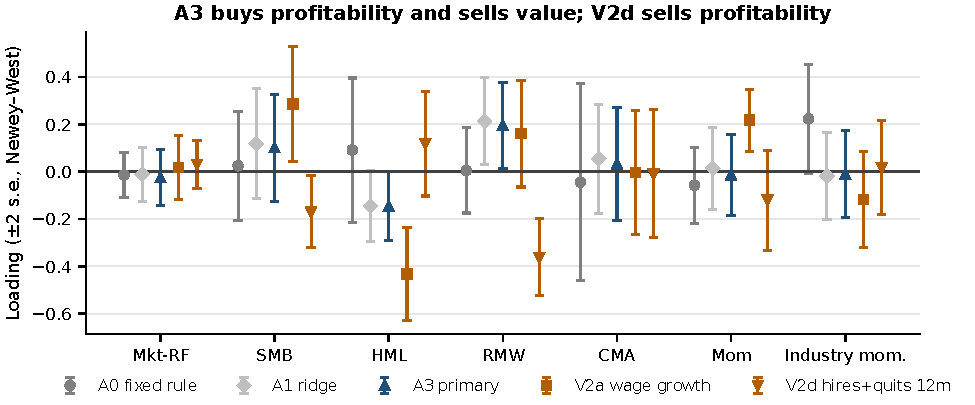
\includegraphics[width=0.92\linewidth]{figures/fig_loadings.pdf}
\caption{Factor loadings of the long--short books: A3 buys profitability and sells value; V2a sells value and buys momentum; V2d sells profitability. \hfill\tagc\ (A0, A1, A3) / \tagp\ (V2a, V2d)}
\label{fig:loadings}
\end{figure}
\begin{figure}[H]
\centering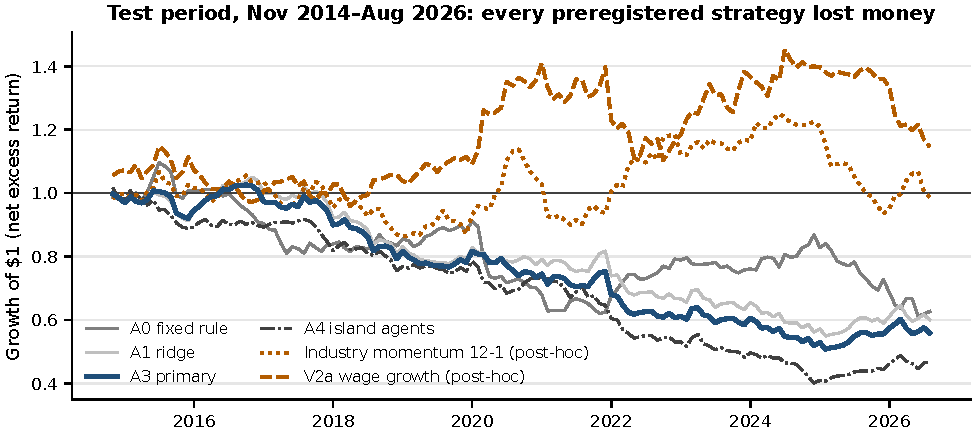
\includegraphics[width=0.92\linewidth]{figures/fig_cumulative.pdf}
\caption{Every preregistered strategy lost money in the test; the post-hoc wage-growth book gained until 2024 and gave much of it back. \hfill\tagc\ (A0--A4) / \tagp\ (momentum, V2a)}
\label{fig:cumulative}
\end{figure}
\begin{figure}[H]
\centering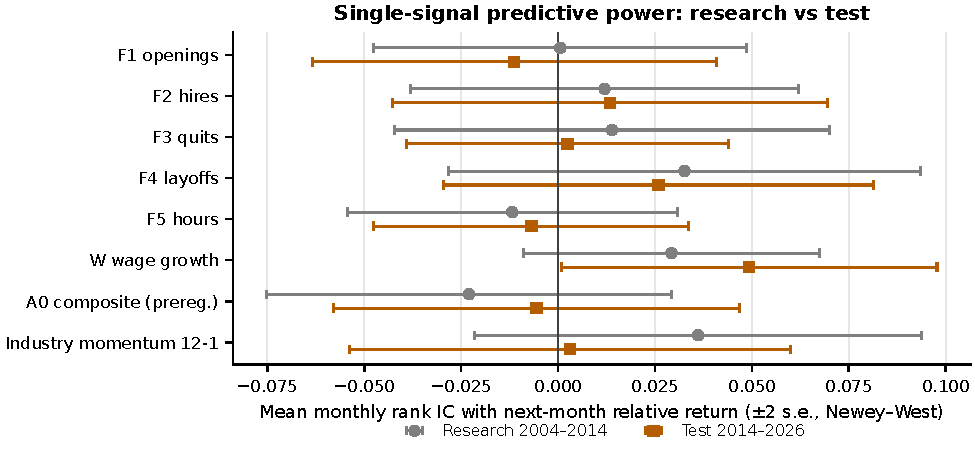
\includegraphics[width=0.92\linewidth]{figures/fig_ic_signals.pdf}
\caption{Only wage growth has a positive IC in both periods; layoffs and hours carry the opposite sign to the one the fixed rule imposed. \hfill\tagp}
\label{fig:ic_signals}
\end{figure}
\begin{figure}[H]
\centering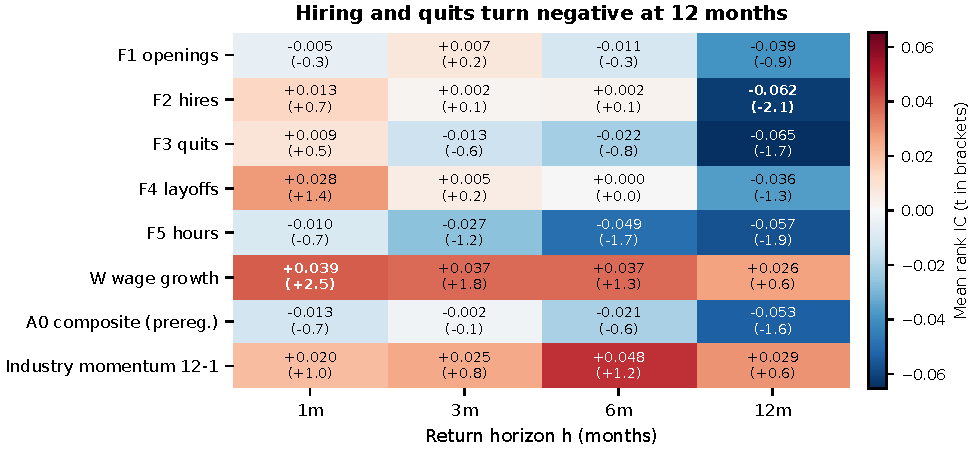
\includegraphics[width=0.86\linewidth]{figures/fig_horizon.pdf}
\caption{Hires and quits turn negative at 12 months ($t=-2.1$, $-1.7$): the investment channel shows up slowly, not within a month. \hfill\tagp}
\label{fig:horizon}
\end{figure}
\begin{figure}[H]
\centering
\begin{subfigure}[t]{0.48\linewidth}\centering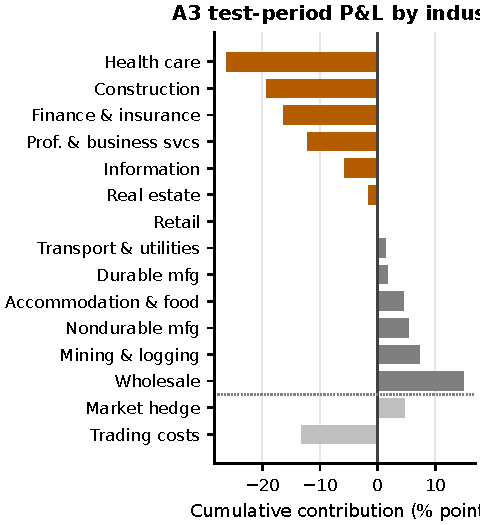
\includegraphics[width=\linewidth]{figures/fig_industry_pnl.pdf}\end{subfigure}\hfill
\begin{subfigure}[t]{0.48\linewidth}\centering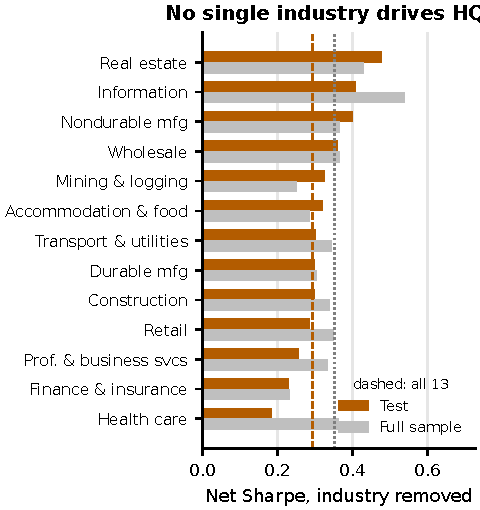
\includegraphics[width=\linewidth]{figures/fig_v2d_dropone.pdf}\end{subfigure}
\caption{Left: the primary lost most in health care, construction and finance. Right: no single industry carries V2d; removing any one leaves its test Sharpe between $+0.18$ and $+0.48$. \hfill\tagp}
\label{fig:pnl_dropone}
\end{figure}
\begin{figure}[H]
\centering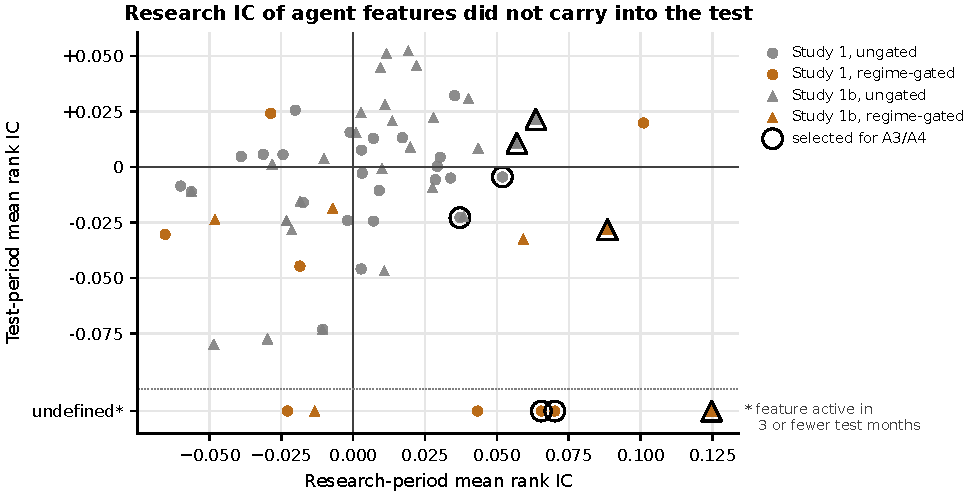
\includegraphics[width=0.92\linewidth]{figures/fig_agents_scatter.pdf}
\caption{Research IC of agent features barely predicts their test IC; the selected regime-gated features were active in 3 test months. \hfill\tagp}
\label{fig:agents_scatter}
\end{figure}
\begin{figure}[H]
\centering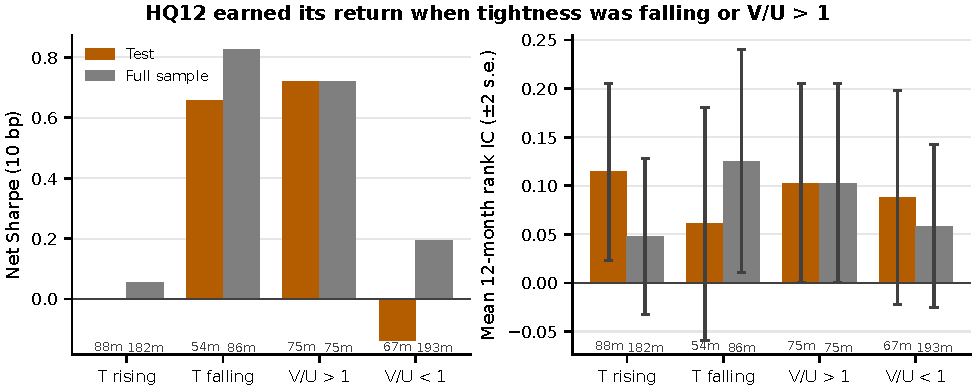
\includegraphics[width=0.92\linewidth]{figures/fig_v2d_tightness.pdf}
\caption{V2d conditional on tightness at the decision: it earned its return when tightness was falling or $V/U>1$; the pattern rests on 54 to 88 months per cell. \hfill\tagp}
\label{fig:v2d_tightness}
\end{figure}
\begin{figure}[H]
\centering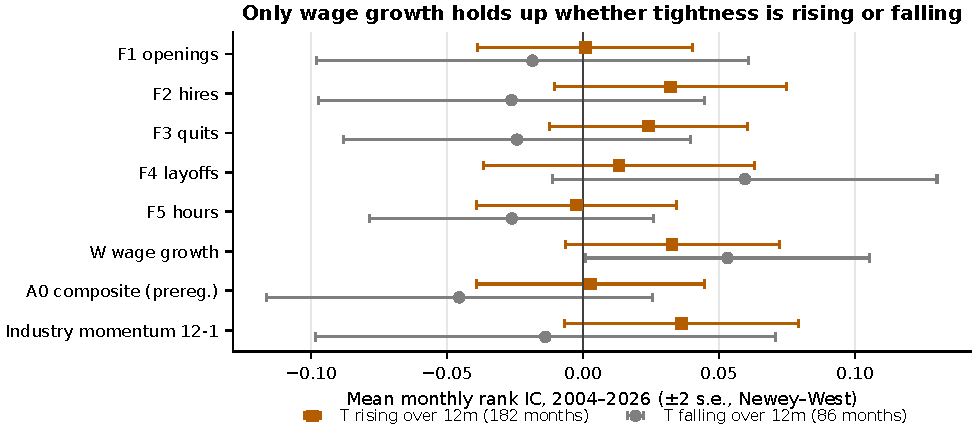
\includegraphics[width=0.92\linewidth]{figures/fig_tightness.pdf}
\caption{Single-signal IC in months when $T$ rose versus fell over the previous 12 months; the split is balanced in both periods. \hfill\tagp}
\label{fig:tightness}
\end{figure}
\begin{table}[H]\centering\footnotesize\caption{Rank IC by horizon, May 2004--August 2026 ($t$ in brackets). \hfill\tagp}\setlength{\tabcolsep}{4pt}% POST-HOC | source: analysis/output/study1/tables/d2_horizon_ic.csv (generated by analysis/run.ipynb)
\begin{tabular}{lrrrr}
\toprule
Signal & 1m & 3m & 6m & 12m \\
\midrule
F1 openings & $-$0.005 ($-$0.31) & +0.007 (+0.23) & $-$0.011 ($-$0.28) & $-$0.039 ($-$0.92) \\
F2 hires & +0.013 (+0.70) & +0.002 (+0.07) & +0.002 (+0.08) & $-$0.062 ($-$2.08) \\
F3 quits & +0.009 (+0.50) & $-$0.013 ($-$0.55) & $-$0.022 ($-$0.78) & $-$0.065 ($-$1.73) \\
F4 layoffs & +0.028 (+1.37) & +0.005 (+0.17) & +0.000 (+0.01) & $-$0.036 ($-$1.28) \\
F5 hours & $-$0.010 ($-$0.67) & $-$0.027 ($-$1.24) & $-$0.049 ($-$1.69) & $-$0.057 ($-$1.86) \\
W wage growth & +0.039 (+2.51) & +0.037 (+1.77) & +0.037 (+1.28) & +0.026 (+0.63) \\
A0 composite (prereg.) & $-$0.013 ($-$0.69) & $-$0.002 ($-$0.09) & $-$0.021 ($-$0.61) & $-$0.053 ($-$1.58) \\
Industry momentum 12-1 & +0.020 (+0.99) & +0.025 (+0.80) & +0.048 (+1.24) & +0.029 (+0.63) \\
\bottomrule
\end{tabular}
\end{table}
\begin{table}[H]\centering\footnotesize\caption{V2d robustness battery: holding period (R3) and sub-periods (R4). \hfill\tagp}\setlength{\tabcolsep}{4pt}% POST-HOC | source: analysis/output/study2/tables/v3_r3_holding.csv (generated by analysis/run.ipynb)
\begin{tabular}{lrrrrrr}
\toprule
Holding & research & test & full & post-2010 & last 18m & Test turnover \\
\midrule
6 months & +0.31 & +0.05 & +0.15 & +0.05 & +0.50 & 0.49 \\
9 months & +0.43 & +0.14 & +0.24 & +0.16 & +0.29 & 0.40 \\
12 months & +0.50 & +0.29 & +0.35 & +0.30 & +0.29 & 0.37 \\
18 months & +0.58 & +0.30 & +0.38 & +0.34 & +0.31 & 0.28 \\
\bottomrule
\end{tabular}
\par\medskip% POST-HOC | source: analysis/output/tables/v3_r4_subperiods.csv (generated by analysis/run.ipynb)
\begin{tabular}{lrrrr}
\toprule
Window & Months & Sharpe & Net p.a. & IC 12m (t) \\
\midrule
test: first half & 71 & $-$0.21 & $-$1.4\% & +0.097 (+1.75) \\
test: second half & 71 & +0.64 & +6.5\% & +0.095 (+1.60) \\
test: excl. Mar 2020-Dec 2021 & 120 & +0.37 & +3.0\% & +0.105 (+2.23) \\
test: pre-2020 & 62 & +0.14 & +0.8\% & +0.114 (+1.92) \\
test: 2020 onward & 80 & +0.37 & +3.9\% & +0.080 (+1.54) \\
full: first half & 134 & +0.33 & +2.0\% & +0.038 (+0.73) \\
full: second half & 134 & +0.38 & +3.3\% & +0.107 (+2.66) \\
full: excl. Mar 2020-Dec 2021 & 246 & +0.40 & +2.9\% & +0.073 (+1.93) \\
full: pre-2020 & 188 & +0.36 & +2.2\% & +0.068 (+1.57) \\
\bottomrule
\end{tabular}
\end{table}

\section{Code snippets}\label{app:code}
\paragraph{As-of lookup} The value of a series known on a cutoff date (frozen \path{data.py}).
\lstinputlisting{code/asof_lookup.py}
\paragraph{Signal construction} Fixed-lag signals and tightness (\path{analysis/data.py}).
\lstinputlisting{code/signals.py}
\paragraph{Backtest core} Tranche, hedge, scaling and costs (frozen \path{data.py}, excerpt).
\lstinputlisting{code/backtest_core.py}

\section{Follow-up study with a stronger model}\label{app:opus}
After the test had been opened, the agent experiment was rerun with Claude Opus~5.5 at extra-high effort, with fresh agents and the same frozen evaluator, selection rule and portfolio. Because the test period was already known to the team, the run is exploratory. Its research-selected primary, A4, earned a test Sharpe of $+0.01$ (research $-0.40$) with an IC of $-0.002$ ($t=-0.10$), an alpha $t$ of 0.05, a placebo $p$ of 0.56 and a Sharpe of $-0.19$ at 25\,bp; it failed gates G2 to G5 and lost 1.41 over the last 18 months. % src: claims X01, X02
Its gross return came from one long position: durable manufacturing contributed $+0.27$ of cumulative return in a group that is 60\% semiconductors. % src: claims X04, S03
Opus's other strategy, A3, earned $-0.46$. % src: claim X03
The follow-up is evidence about agents (\cref{sec:claude}), not about the strategy.

\section{Forward-test specification}\label{app:forward}
\begin{itemize}
  \item \path{analysis/v2_spec.md}: four post-hoc variants and a reading rule; SHA-256 \texttt{ca658234\ldots}, frozen 2026-10-03T09:00:13Z, first run 09:01:55Z. % src: claim F08; analysis/output/v2_run_log.md
  \item \path{analysis/forward/spec_frozen.md}: decision 30 September 2026, information cutoff 29 September, one tranche held to 31 December, 60-month beta hedge in SPY, 10\,bp and 2\,bp costs; SHA-256 \texttt{735a8ffa\ldots}, frozen 09:03:56Z. % src: claims F08, F05
  \item \path{analysis/forward/spec_amendment_001.md}: the fixed-lag information set (JOLTS July 2026, CES August 2026, as published on 29 September) after the pre-committed check stopped the first run; V2c and V2d added after the historical v2 results were seen and before any Q4 return beyond 1--2 October; SHA-256 \texttt{c76cde86\ldots}, frozen 09:16:11Z; book built 09:17:55Z. % src: claims F08, F05
  \item \path{analysis/v3_spec.md}: the robustness battery; SHA-256 \texttt{312aef1d\ldots}, frozen 09:52:27Z, first run 09:53:32Z. % src: claim F08; analysis/output/v3_run_log.md
  \item Books: \path{analysis/forward/book_2026Q4.csv} (group weights for V2a--V2d), \path{book_2026Q4_etf.csv} (netted ETF weights), \path{book_2026Q4_hedge.csv} (SPY hedge per unit: $-0.40$, $-0.06$, $-0.24$, $-0.02$), % src: claim F03
  \path{etf_proxies.csv}. V2b is long durable manufacturing, retail and transport and short real estate, health care and accommodation; V2c is long construction, durable manufacturing and finance and short retail, transport and professional services. % src: claims F06, F07
  \item Evaluation: the ETF books from the 30 September close to the 31 December close after costs, and the same books on Ken French group returns once published; reported whatever they show. \todo{Elouan: weekly tracker (deferred by team decision)}
\end{itemize}

\end{document}
